\documentclass{article}
\usepackage{xcolor}
\usepackage{titleps}
\usepackage[letterpaper, margin=0.95in]{geometry}
\usepackage{url}
\usepackage{amsmath}
\usepackage{amssymb}
\usepackage{wrapfig}
\usepackage{float}
\usepackage{mathtools}
\usepackage{enumitem}
\usepackage{tabu}
\usepackage{parskip}
\usepackage{natbib}
\usepackage{listings}

\usepackage[many]{tcolorbox}
\usepackage{minted}
\setminted[python]{
	% frame=single,
	% linenos,
    xleftmargin=0.475em,
    baselinestretch=1.2,
}
% https://tex.stackexchange.com/a/569249
\setcounter{secnumdepth}{5}
\setcounter{tocdepth}{5}
\makeatletter
\newcommand\subsubsubsection{\@startsection{paragraph}{4}{\z@}{-2.5ex\@plus -1ex \@minus -.25ex}{1.25ex \@plus .25ex}{\normalfont\normalsize\bfseries}}
\newcommand\subsubsubsubsection{\@startsection{subparagraph}{5}{\z@}{-2.5ex\@plus -1ex \@minus -.25ex}{1.25ex \@plus .25ex}{\normalfont\normalsize\bfseries}}
\makeatother

\usepackage{hyperref}
\usepackage[color=red]{todonotes}
\usepackage{forest}
\definecolor{light-yellow}{HTML}{FFE5CC}

\newpagestyle{ruled}
{\sethead{CMU 16-831}{Introduction to Robot Learning }{Spring 2024}\headrule
  \setfoot{}{}{}}
\pagestyle{ruled}

\renewcommand\makeheadrule{\color{black}\rule[-.75\baselineskip]{\linewidth}{0.4pt}}
\renewcommand*\footnoterule{}

\newtcolorbox[]{answer}[1][]{
    % breakable,
    enhanced,
    nobeforeafter,
    colback=white,
    title=Your Answer,
    sidebyside align=top,
    box align=top,
    #1
}



\begin{document}

\lstset{basicstyle = \ttfamily,columns=fullflexible,
    backgroundcolor = \color{light-yellow}
}

\begin{centering}
    {\Large Assignment 4: Model-Based RL and Exploration
    } \\
    \vspace{.25cm}
\end{centering}
\vspace{0.25cm}

\textbf{Andrew ID:} \texttt{mukaiy} \\
% \textbf{Collaborators:} \texttt{Write the Andrew IDs of your collaborators here (if any).}\\
\textbf{NOTE:} Please do \textbf{NOT} change the sizes of the answer blocks or plots.

\section{Problem 1: Dynamics Model Training -- \lbrack10 points total\rbrack}
\begin{answer}[title=Theory questions,height=4.5cm,width=\linewidth]
    The third model performs the best, because it achieves the least $MPE = 0.07804489$.

    More training steps per iteration improves convergence a lot, and larger MLP interpolates better.
\end{answer}


\begin{answer}[title=Plot,height=9.5cm,width=\linewidth]
    % TODO
    \begin{figure}[H]
        \centering
        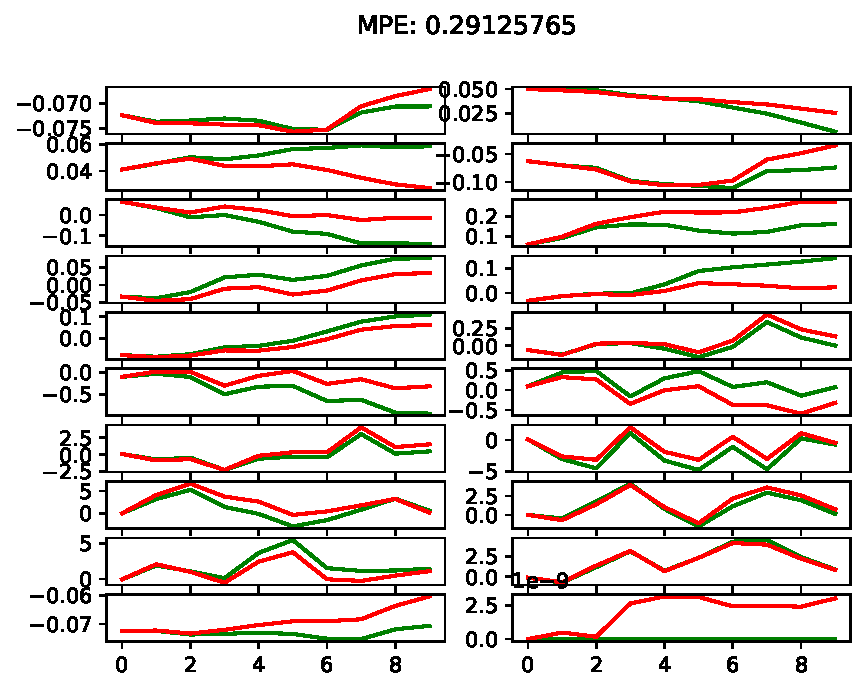
\includegraphics[height=7cm]{figs/P1_1.pdf}
        \caption{500 training steps per iteration, 1 x 32 MLP.}
    \end{figure}
\end{answer}

\begin{answer}[title=Plot,height=9.5cm,width=\linewidth]
    % TODO
    \begin{figure}[H]
        \centering
        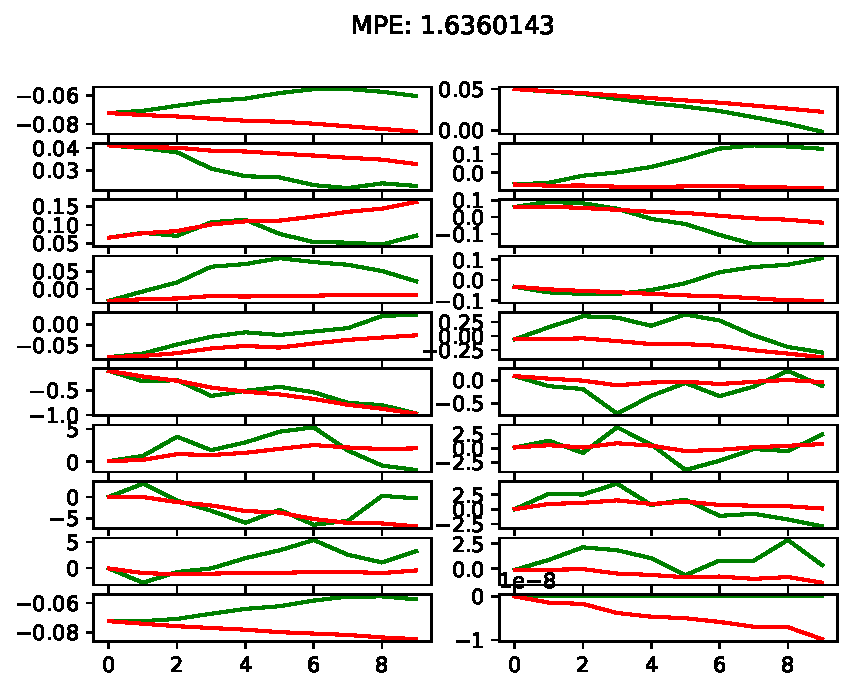
\includegraphics[height=7cm]{figs/P1_2.pdf}
        \caption{5 training steps per iteration, 2 x 250 MLP.}
    \end{figure}
\end{answer}

\begin{answer}[title=Plot,height=9.5cm,width=\linewidth]
    % TODO
    \begin{figure}[H]
        \centering
        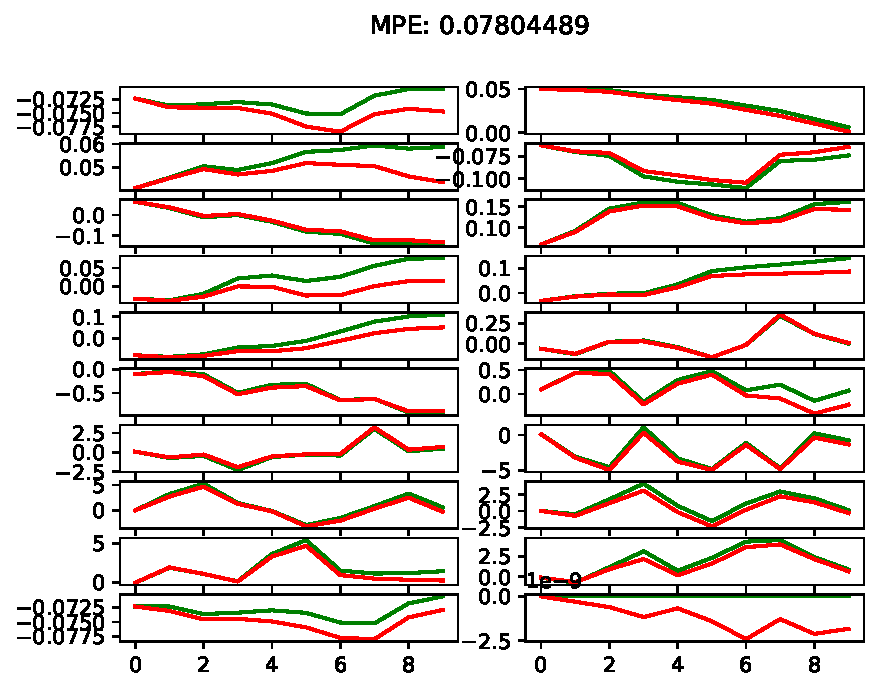
\includegraphics[height=7cm]{figs/P1_3.pdf}
        \caption{500 training steps per iteration, 2 x 250 MLP.}
    \end{figure}
\end{answer}

\section{Problem 2: Action Selection}
\begin{answer}[title=Plot,height=9.5cm,width=\linewidth]
    % TODO
    \begin{figure}[H]
        \centering
        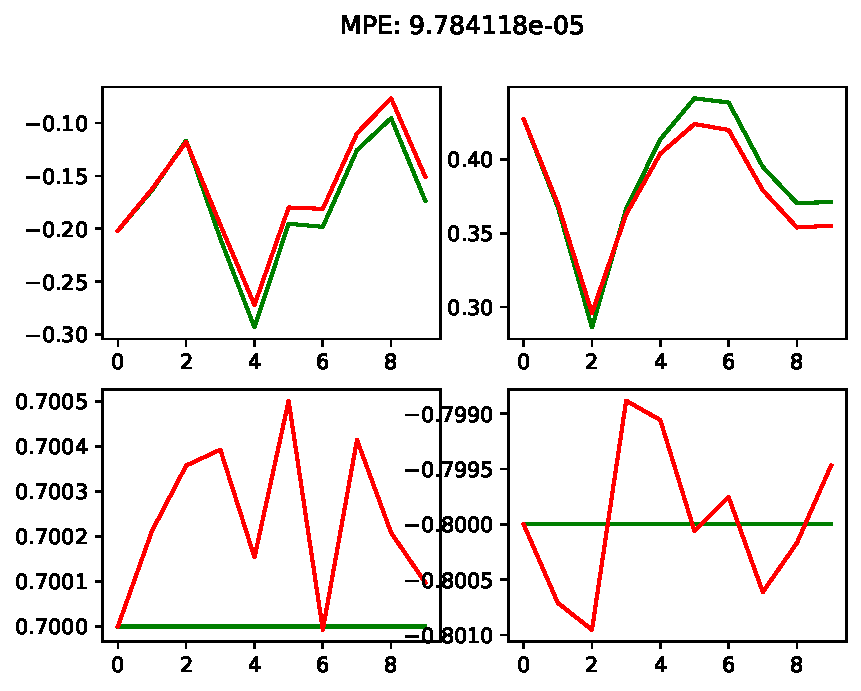
\includegraphics[height=7cm]{figs/P2.pdf}
        \caption{Optimizing the Dynamics Model where MPC needs to be used improves a lot.}
    \end{figure}
\end{answer}



\section{Problem 3: Iterative Model Training}
\begin{answer}[title=Plot,height=9.5cm,width=\linewidth]
    % TODO
    \centering
    \includegraphics[height=8cm]{example-image-a}
\end{answer}

\begin{answer}[title=Plot,height=9.5cm,width=\linewidth]
    % TODO
    \centering
    \includegraphics[height=8cm]{example-image-a}
\end{answer}

\begin{answer}[title=Plot,height=9.5cm,width=\linewidth]
    % TODO
    \centering
    \includegraphics[height=8cm]{example-image-a}
\end{answer}

\section{Problem 4: Hyper-parameter Comparison}
\begin{answer}[title=Plot,height=9.5cm,width=\linewidth]
    % TODO
    \centering
    \includegraphics[height=8cm]{example-image-a}
\end{answer}

\begin{answer}[title=Plot,height=9.5cm,width=\linewidth]
    % TODO
    \centering
    \includegraphics[height=8cm]{example-image-a}
\end{answer}

\begin{answer}[title=Plot,height=9.5cm,width=\linewidth]
    % TODO
    \centering
    \includegraphics[height=8cm]{example-image-a}
\end{answer}


\section{Problem 5: Hyper-parameter Comparison (Bonus)}
\begin{answer}[title=Plot,height=9.5cm,width=\linewidth]
    % TODO
    \centering
    \includegraphics[height=8cm]{example-image-a}
\end{answer}


\section{Problem 6: Exploration (Bonus)}
\begin{answer}[title=Plot,height=9.5cm,width=\linewidth]
    % TODO
    \centering
    \includegraphics[height=8cm]{example-image-a}
\end{answer}

\begin{answer}[title=Plot,height=9.5cm,width=\linewidth]
    % TODO
    \centering
    \includegraphics[height=8cm]{example-image-a}
\end{answer}

\begin{answer}[title=Plot,height=9.5cm,width=\linewidth]
    % TODO
    \centering
    \includegraphics[height=8cm]{example-image-a}
\end{answer}

\begin{answer}[title=Plot,height=9.5cm,width=\linewidth]
    % TODO
    \centering
    \includegraphics[height=8cm]{example-image-a}
\end{answer}


\end{document}
